% Meridian Link Whitepaper
% Professional LaTeX Document
\documentclass[11pt,a4paper,twoside]{article}

% ============================================================================
% PACKAGES
% ============================================================================
\usepackage[utf8]{inputenc}
\usepackage[T1]{fontenc}
\usepackage{lmodern}
\usepackage[margin=1in]{geometry}
\usepackage{graphicx}
\usepackage{xcolor}
\usepackage{hyperref}
\usepackage{amsmath,amssymb,amsthm}
\usepackage{booktabs}
\usepackage{longtable}
\usepackage{array}
\usepackage{multirow}
\usepackage{enumitem}
\usepackage{fancyhdr}
\usepackage{titlesec}
\usepackage{tocloft}
\usepackage{listings}
\usepackage{tikz}
\usepackage{pgfplots}
\usepackage{caption}
\usepackage{subcaption}
\usepackage{float}
\usepackage{setspace}
\usepackage{parskip}
% Using manual references instead of biblatex for compatibility

\usetikzlibrary{shapes.geometric, arrows.meta, positioning, fit, backgrounds, calc}
\pgfplotsset{compat=1.18}

% ============================================================================
% COLORS
% ============================================================================
\definecolor{primaryblue}{RGB}{26, 54, 93}
\definecolor{accentblue}{RGB}{59, 130, 246}
\definecolor{darkgray}{RGB}{55, 65, 81}
\definecolor{lightgray}{RGB}{243, 244, 246}
\definecolor{codebg}{RGB}{249, 250, 251}
\definecolor{solanagreen}{RGB}{20, 241, 149}
\definecolor{ethereumblue}{RGB}{98, 126, 234}

% ============================================================================
% HYPERREF SETUP
% ============================================================================
\hypersetup{
    colorlinks=true,
    linkcolor=primaryblue,
    citecolor=accentblue,
    urlcolor=accentblue,
    pdftitle={Meridian Link: Trust-Minimized Cross-Chain Token Transfers},
    pdfauthor={Jayanth Kumar Morem},
    pdfsubject={Cross-Chain Bridge Whitepaper},
    pdfkeywords={blockchain, cross-chain, zero-knowledge proofs, Solana, Ethereum, ZK compression}
}

% ============================================================================
% HEADER/FOOTER
% ============================================================================
\pagestyle{fancy}
\fancyhf{}
\fancyhead[LE,RO]{\thepage}
\fancyhead[RE]{\textit{Meridian Link Whitepaper}}
\fancyhead[LO]{\textit{\nouppercase{\leftmark}}}
\renewcommand{\headrulewidth}{0.4pt}
\fancypagestyle{plain}{
    \fancyhf{}
    \fancyfoot[C]{\thepage}
    \renewcommand{\headrulewidth}{0pt}
}

% ============================================================================
% SECTION FORMATTING
% ============================================================================
\titleformat{\section}
    {\normalfont\Large\bfseries\color{primaryblue}}
    {\thesection}{1em}{}
\titleformat{\subsection}
    {\normalfont\large\bfseries\color{darkgray}}
    {\thesubsection}{1em}{}
\titleformat{\subsubsection}
    {\normalfont\normalsize\bfseries\color{darkgray}}
    {\thesubsubsection}{1em}{}

% ============================================================================
% TABLE OF CONTENTS
% ============================================================================
\renewcommand{\cftsecfont}{\bfseries\color{primaryblue}}
\renewcommand{\cftsecpagefont}{\bfseries\color{primaryblue}}
\renewcommand{\cftsubsecfont}{\color{darkgray}}

% ============================================================================
% CODE LISTINGS
% ============================================================================
\lstdefinestyle{code}{
    backgroundcolor=\color{codebg},
    basicstyle=\ttfamily\small,
    breakatwhitespace=false,
    breaklines=true,
    captionpos=b,
    keepspaces=true,
    numbers=none,
    showspaces=false,
    showstringspaces=false,
    showtabs=false,
    tabsize=2,
    frame=single,
    rulecolor=\color{lightgray},
    xleftmargin=0.5em,
    xrightmargin=0.5em,
}
\lstset{style=code}

% ============================================================================
% CUSTOM COMMANDS
% ============================================================================
\newcommand{\protocol}{\textsc{Meridian Link}}
\newcommand{\poseidon}{\textsc{Poseidon}}
\newcommand{\groth}{\textsc{Groth16}}

% ============================================================================
% DOCUMENT
% ============================================================================
\begin{document}

% ============================================================================
% TITLE PAGE
% ============================================================================
\begin{titlepage}
    \begin{center}
        \vspace*{2cm}
        
        {\Huge\bfseries Meridian Link}
        
        \vspace{0.8cm}
        
        {\Large Trust-Minimized Cross-Chain Token Transfers\\[0.3cm]Between Solana and EVM Chains via ZK Compression}
        
        \vspace{1.5cm}
        
        {\large\textbf{Jayanth Kumar Morem}}
        
        \vspace{0.3cm}
        
        {\normalsize\texttt{jayanthkumar1903@gmail.com}}
        
        \vspace{2cm}
        
        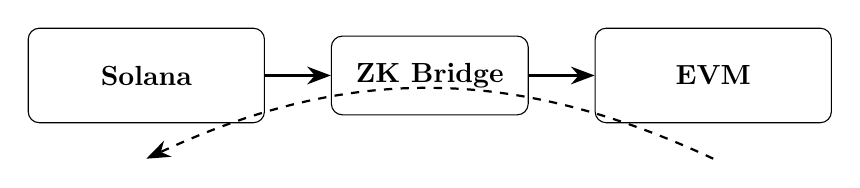
\begin{tikzpicture}[scale=0.9]
            % Solana node
            \node[draw, rounded corners, minimum width=3cm, minimum height=1.2cm] (solana) at (-4,0) {\textbf{Solana}};
            % Bridge
            \node[draw, rounded corners, minimum width=2.5cm, minimum height=1cm] (bridge) at (0,0) {\textbf{ZK Bridge}};
            % EVM node  
            \node[draw, rounded corners, minimum width=3cm, minimum height=1.2cm] (evm) at (4,0) {\textbf{EVM}};
            % Arrows
            \draw[-{Stealth[length=3mm]}, thick] (solana) -- (bridge);
            \draw[-{Stealth[length=3mm]}, thick] (bridge) -- (evm);
            \draw[-{Stealth[length=3mm]}, thick, dashed] ([yshift=-0.5cm]evm.south) to[bend right=25] ([yshift=-0.5cm]solana.south);
        \end{tikzpicture}
        
        \vspace{2.5cm}
        
        {\large Version 1.0}
        
        \vspace{0.5cm}
        
        {\large January 2026}
        
        \vfill
        
        \begin{tabular}{c}
            \textit{Technical Whitepaper}\\[0.3cm]
            \url{https://github.com/RippnerLabs/meridian-link}
        \end{tabular}
        
    \end{center}
\end{titlepage}

% ============================================================================
% ABSTRACT
% ============================================================================
\newpage
\begin{abstract}
\noindent
Cross-chain bridges represent one of the most critical yet vulnerable components of blockchain infrastructure, with over \$2.5 billion lost to bridge exploits between 2022--2023 alone. \protocol{} introduces an architecture combining Light Protocol's ZK Compression on Solana with \groth{} zero-knowledge proofs for verification on EVM chains, reducing trust assumptions compared to signature-based bridges while acknowledging explicit trade-offs.

\vspace{0.5cm}
\noindent\textbf{Key Properties:}
\begin{itemize}[noitemsep,topsep=0pt]
    \item \textbf{Cost reduction:} 95\%+ savings on Solana storage via compressed accounts ($\sim$15,000 vs $\sim$1,600,000 lamports per deposit record)
    \item \textbf{Verification:} \groth{} proofs ($\sim$100-bit security on BN254) replace multisig attestation for withdrawal authorization
    \item \textbf{Latency:} $\sim$20--25 seconds end-to-end (competitive with intent-based bridges)
    \item \textbf{Replay protection:} \poseidon{}-based nullifiers with on-chain tracking
\end{itemize}

\vspace{0.5cm}
\noindent\textbf{Explicit Limitations:}
\begin{itemize}[noitemsep,topsep=0pt]
    \item \textbf{Throughput:} $\sim$12--20 withdrawals per minute per direction (sequential IMT updates)
    \item \textbf{EVM costs:} Withdrawal verification costs $\sim$\$4--6 at 30 gwei, dominating total transfer cost
    \item \textbf{Trust assumptions:} \groth{} trusted setup, Light Protocol implementation, Photon indexer availability, relayer liveness
\end{itemize}

\vspace{0.5cm}
\noindent
The protocol shifts the trust model from ``honest majority of signers'' to ``cryptographic soundness plus infrastructure liveness.'' A compromised relayer cannot forge proofs or double-spend, but can censor transactions or extract MEV through reordering.
\end{abstract}

% ============================================================================
% TABLE OF CONTENTS
% ============================================================================
\newpage
\tableofcontents
\newpage

% ============================================================================
% SECTION 1: PROBLEM STATEMENT
% ============================================================================
\section{Problem Statement}
\label{sec:problem}

Cross-chain bridges face three fundamental challenges that current solutions fail to adequately address.

\subsection{Prohibitive On-Chain Storage Costs}

Most bridges store transaction records directly on-chain, incurring substantial storage costs that scale linearly with usage. On Solana, creating a standard Program Derived Account (PDA) requires approximately 1,600,000 lamports ($\sim$\$0.25 at current prices) for rent-exemption of a 100-byte account~[1]. For a bridge processing thousands of transactions daily, these costs become economically prohibitive.

\textbf{\protocol{}'s approach:} By leveraging Light Protocol's state compression, we reduce storage costs by over 95\%. A compressed account costs approximately 15,000 lamports versus 1,600,000 lamports for a traditional PDA,a 99.06\% reduction~[2]. This is achieved by storing only a 32-byte hash of the account data in a sparse Merkle tree, with the full account data recorded on the Solana ledger (not in expensive account space).

\begin{table}[H]
\centering
\caption{Storage Cost Comparison}
\label{tab:storage-costs}
\begin{tabular}{@{}lccc@{}}
\toprule
\textbf{Account Type} & \textbf{Traditional Cost} & \textbf{Compressed Cost} & \textbf{Savings} \\
\midrule
Token Account & $\sim$2,000,000 lamports & $\sim$5,000 lamports & 99.75\% \\
100-byte PDA & $\sim$1,600,000 lamports & $\sim$15,000 lamports & 99.06\% \\
Nullifier PDA & $\sim$890,880 lamports & $\sim$15,000 lamports & 98.32\% \\
\bottomrule
\end{tabular}
\end{table}

\subsection{Trust in Intermediaries}

Existing bridges require users to trust various intermediaries:

\begin{itemize}
    \item \textbf{Multisig committees:} Wormhole's Guardian Network requires 13-of-19 guardians to attest to cross-chain messages~[3]. A compromise of 7 guardians enables arbitrary message forgery.
    \item \textbf{Oracle networks:} LayerZero's Decentralized Verifier Networks (DVNs) introduce oracle trust assumptions~[4].
    \item \textbf{Liquidity providers:} Pool-based bridges like Allbridge require trust in pool operators and expose users to impermanent loss.
\end{itemize}

\textbf{\protocol{}'s approach:} We employ \groth{} zk-SNARK proofs~[5] for verification, reducing trust to cryptographic assumptions. The withdrawal of tokens on the destination chain requires a valid zero-knowledge proof demonstrating that:
\begin{enumerate}
    \item A corresponding deposit exists on the source chain
    \item The deposit is included in the protocol's state tree
    \item The nullifier has not been previously used (preventing double-spending)
\end{enumerate}

The relayer cannot forge proofs,computational infeasibility under the discrete logarithm assumption on BN254 ($\sim$100-bit security). However, trust assumptions remain:
\begin{itemize}
    \item \textbf{Trusted setup:} \groth{} requires a circuit-specific ceremony; a compromised setup enables proof forgery
    \item \textbf{Liveness:} The relayer must be operational; if it fails, users reclaim deposits via time-lock mechanism
    \item \textbf{Infrastructure:} Light Protocol and Photon indexer must function correctly
\end{itemize}

\subsection{Replay Attacks and Double-Spending}

Without proper replay protection, a single deposit could be used to withdraw tokens multiple times. Many bridges rely on centralized tracking systems that introduce single points of failure.

\textbf{\protocol{}'s approach:} Each bridge request generates a unique nullifier computed via \poseidon{} hashing~[6]:

\begin{equation}
\text{nullifier} = \poseidon_7(\text{depId}, \text{srcChain}, \text{destChain}, \text{amt}, \text{mint}, \text{owner}, \text{ts})
\end{equation}

This nullifier is:
\begin{itemize}
    \item Computed deterministically from the deposit parameters (cannot be guessed or forged)
    \item Stored on-chain after each withdrawal (preventing reuse)
    \item Verified as part of the zero-knowledge proof (cryptographically bound to the deposit)
\end{itemize}

The \poseidon{} hash function is specifically chosen for its efficiency in arithmetic circuits, requiring only $\sim$300 constraints per hash operation compared to $\sim$25,000 for SHA-256~[7].

% ============================================================================
% SECTION 2: WHY BRIDGING IS HARD
% ============================================================================
\section{Why Solana $\leftrightarrow$ EVM Bridging is Hard}
\label{sec:challenges}

Cross-chain communication between Solana and EVM chains presents unique technical challenges that distinguish it from bridging between homogeneous blockchain families.

\subsection{Consensus Incompatibility}

Solana employs a hybrid consensus mechanism combining Proof of History (PoH) with Tower BFT~[8]:
\begin{itemize}
    \item \textbf{Slot time:} 400ms
    \item \textbf{Processed commitment:} Transaction received by leader ($\sim$400ms)
    \item \textbf{Confirmed commitment:} Supermajority (66\%+) vote confirmation ($\sim$2--3 seconds)
    \item \textbf{Finalized commitment:} 31+ confirmed blocks built atop ($\sim$15--30 seconds)
\end{itemize}

Ethereum (post-Merge) uses Gasper consensus~[9]:
\begin{itemize}
    \item \textbf{Block time:} 12 seconds
    \item \textbf{Epoch:} 32 slots (6.4 minutes)
    \item \textbf{Finality:} 2 epochs ($\sim$12.8 minutes under normal conditions)
\end{itemize}

There is no native mechanism for one chain to verify the consensus of the other. Light client implementations would require:
\begin{itemize}
    \item Solana to verify Ethereum's BLS aggregate signatures over the validator set
    \item Ethereum to verify Solana's Tower BFT votes and PoH chain
\end{itemize}

Neither chain natively supports the cryptographic primitives required for the other's consensus verification, making true trustless light clients impractical without significant protocol changes.

\subsection{Address Space and Field Constraints}

\textbf{Circom's field limitation:} Zero-knowledge circuits in Circom operate over the BN254 (alt\_bn128) elliptic curve scalar field, which has a prime order of approximately $2^{254}$~[10]. This creates challenges when handling:

\begin{itemize}
    \item \textbf{Ethereum addresses:} 160 bits (20 bytes) , fits within the field
    \item \textbf{Solana addresses:} 256 bits (32 bytes) , exceeds the field size
\end{itemize}

\textbf{\protocol{}'s solution:} For the Ethereum Deposit Proof circuit, we split 256-bit values into two 128-bit chunks:

\begin{lstlisting}[language=C,caption={Address Splitting in Circom}]
signal input depositorHigh;  // Upper 128 bits
signal input depositorLow;   // Lower 128 bits
\end{lstlisting}

\subsection{Transaction Size Constraints}

Solana enforces a strict 1,232-byte limit on transaction size~[11]. A typical cross-chain withdrawal transaction must include:
\begin{itemize}
    \item \groth{} proof: 256 bytes (compressed)
    \item Public inputs: $\sim$128 bytes
    \item Merkle proof path: Variable (up to 832 bytes for 26 levels)
    \item Account metadata: $\sim$100 bytes
\end{itemize}

Light Protocol's validity proof optimization reduces the Merkle proof requirement to a constant 128 bytes by leveraging the on-chain state root, making cross-chain transactions feasible within Solana's constraints~[2].

\subsection{The Oracle Problem}

Most existing Solana-EVM bridges rely on oracle-based attestation:

\begin{itemize}
    \item \textbf{Wormhole:} 19 Guardian nodes sign observed messages; 13/19 threshold for validity~[3]
    \item \textbf{LayerZero:} Decentralized Verifier Networks (DVNs) attest to cross-chain messages~[4]
\end{itemize}

These approaches inherit the security assumptions of the oracle network. If the oracle set is compromised (via key theft, coercion, or collusion), arbitrary messages can be forged.

\textbf{\protocol{}'s approach:} Rather than trusting oracles to attest to state, we generate cryptographic proofs that the state exists. The security reduces to:
\begin{enumerate}
    \item The soundness of the \groth{} proof system ($\sim$100-bit security)~[5]
    \item The integrity of the on-chain state root (verified by Solana/Ethereum consensus)
    \item The correctness of the circuit (auditable, deterministic)
\end{enumerate}

% ============================================================================
% SECTION 3: EXISTING BRIDGE MODELS
% ============================================================================
\section{Existing Bridge Models}
\label{sec:existing}

\subsection{Wormhole (Portal Bridge)}

\textbf{Architecture:} Lock-and-mint model with Guardian Network attestation~[3]

\begin{itemize}
    \item \textbf{TVL:} $\sim$\$2 billion (as of 2024)
    \item \textbf{Trust model:} 19 Guardian nodes operated by institutional validators; 13/19 threshold
    \item \textbf{Mechanism:}
    \begin{enumerate}
        \item User locks tokens on source chain
        \item Guardians observe and sign VAA (Verified Action Approval)
        \item User submits VAA to destination chain
        \item Destination chain mints wrapped tokens
    \end{enumerate}
\end{itemize}

\textbf{Security incident:} In February 2022, an attacker exploited a signature verification vulnerability, stealing \$326 million in wrapped ETH~[12].

\textbf{Limitations:}
\begin{itemize}
    \item Wrapped tokens introduce additional smart contract risk
    \item Guardian compromise enables arbitrary minting
    \item Latency of 15--20 minutes for finality
\end{itemize}

\subsection{LayerZero}

\textbf{Architecture:} Ultra Light Node (ULN) with configurable security~[4]

\begin{itemize}
    \item \textbf{TVL:} N/A (messaging protocol, not custodial)
    \item \textbf{Trust model:} Oracle + Relayer separation; Decentralized Verifier Networks (DVNs)
    \item \textbf{Mechanism:}
    \begin{enumerate}
        \item Source chain emits message
        \item DVNs verify and sign the message
        \item Relayer submits message to destination
        \item Destination chain verifies DVN signatures
    \end{enumerate}
\end{itemize}

\textbf{Limitations:}
\begin{itemize}
    \item Security depends on DVN selection and configuration
    \item Application developers must choose appropriate security settings
    \item No native support for Solana (requires custom adapters)
\end{itemize}

\subsection{deBridge}

\textbf{Architecture:} Intent-based Deferred Liquidity Network (DLN)~[13]

\begin{itemize}
    \item \textbf{TVL:} Growing (no pooled liquidity model)
    \item \textbf{Trust model:} Authenticated messages via validator signatures
    \item \textbf{Mechanism:}
    \begin{enumerate}
        \item User creates intent (desired outcome)
        \item Solvers compete to fulfill the intent
        \item Settlement occurs via authenticated messages
    \end{enumerate}
\end{itemize}

\textbf{Inspiration for \protocol{}:} deBridge's no-wrapped-token approach and real-time execution model influenced our design. However, deBridge still relies on validator signatures rather than cryptographic proofs.

\subsection{Allbridge Core}

\textbf{Architecture:} Liquidity pool model with native stablecoin transfers~[14]

\begin{itemize}
    \item \textbf{TVL:} $\sim$\$25 million
    \item \textbf{Trust model:} Pool operators and liquidity providers
    \item \textbf{Mechanism:}
    \begin{enumerate}
        \item User deposits tokens into source pool
        \item Equivalent tokens released from destination pool
        \item Pool rebalancing via cross-chain messages
    \end{enumerate}
\end{itemize}

\textbf{Limitations:}
\begin{itemize}
    \item Liquidity fragmentation across pools
    \item Exposure to impermanent loss for LPs
    \item Pool depletion risk during high-volume periods
\end{itemize}

\subsection{Meridian Link Positioning}

\protocol{} differentiates from the above models through ZK proof-based verification rather than signature aggregation, combined with compressed on-chain storage via Light Protocol. A detailed quantitative comparison is provided in Section~\ref{sec:comparison}.

% ============================================================================
% SECTION 4: ARCHITECTURE PROPOSAL
% ============================================================================
\section{Architecture Proposal}
\label{sec:architecture}

\protocol{} consists of five primary components working in concert to enable cross-chain transfers with reduced trust assumptions.

\subsection{System Architecture Overview}

\begin{figure}[H]
\centering
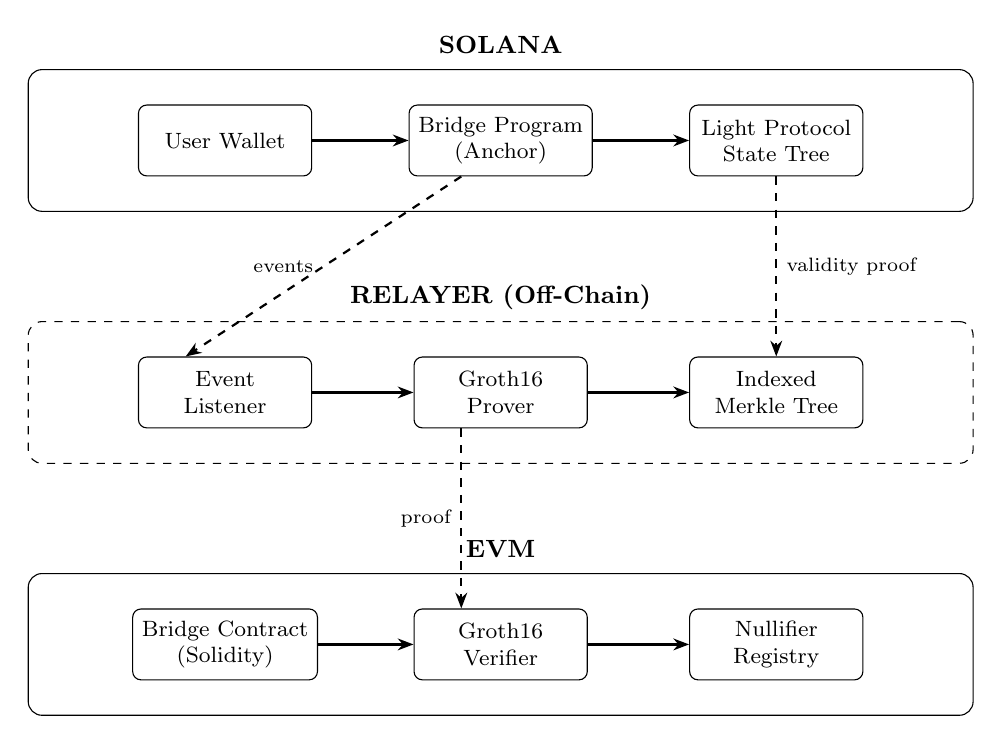
\begin{tikzpicture}[
    node distance=0.8cm,
    component/.style={draw, rounded corners=3pt, minimum width=2.2cm, minimum height=0.9cm, align=center, font=\footnotesize},
    layer/.style={draw, rounded corners=5pt, minimum width=12cm, minimum height=1.8cm},
    arrow/.style={-{Stealth[length=2mm]}, thick},
    label/.style={font=\small\bfseries}
]

% Solana Layer
\node[layer] (sollayer) at (0,6) {};
\node[label] at ([yshift=0.3cm]sollayer.north) {SOLANA};
\node[component] (wallet1) at (-3.5,6) {User Wallet};
\node[component] (solbridge) at (0,6) {Bridge Program\\(Anchor)};
\node[component] (light) at (3.5,6) {Light Protocol\\State Tree};
\draw[arrow] (wallet1) -- (solbridge);
\draw[arrow] (solbridge) -- (light);

% Relayer Layer  
\node[layer, dashed] (rellayer) at (0,2.8) {};
\node[label] at ([yshift=0.3cm]rellayer.north) {RELAYER (Off-Chain)};
\node[component] (listener) at (-3.5,2.8) {Event\\Listener};
\node[component] (prover) at (0,2.8) {Groth16\\Prover};
\node[component] (imt) at (3.5,2.8) {Indexed\\Merkle Tree};
\draw[arrow] (listener) -- (prover);
\draw[arrow] (prover) -- (imt);

% EVM Layer
\node[layer] (evmlayer) at (0,-0.4) {};
\node[label] at ([yshift=0.3cm]evmlayer.north) {EVM};
\node[component] (evmbridge) at (-3.5,-0.4) {Bridge Contract\\(Solidity)};
\node[component] (verifier) at (0,-0.4) {Groth16\\Verifier};
\node[component] (nullifier) at (3.5,-0.4) {Nullifier\\Registry};
\draw[arrow] (evmbridge) -- (verifier);
\draw[arrow] (verifier) -- (nullifier);

% Cross-layer arrows (positioned to left side to avoid label overlap)
\draw[arrow, dashed] ([xshift=-0.5cm]solbridge.south) -- node[left, font=\scriptsize, pos=0.5] {events} ([xshift=-0.5cm]listener.north);
\draw[arrow, dashed] ([xshift=-0.5cm]prover.south) -- node[left, font=\scriptsize, pos=0.5] {proof} ([xshift=-0.5cm]verifier.north);
\draw[arrow, dashed] (light.south) -- node[right, font=\scriptsize, pos=0.5] {validity proof} (imt.north);

\end{tikzpicture}
\caption{Meridian Link System Architecture}
\label{fig:architecture}
\end{figure}

\subsection{Component 1: Solana Bridge Program}

The Solana bridge program is implemented using the Anchor framework and integrates with Light Protocol for state compression.

\subsubsection{Account Structures}

The program maintains four primary account types:

\begin{table}[H]
\centering
\caption{Solana Bridge Account Types}
\label{tab:accounts}
\begin{tabular}{@{}lll@{}}
\toprule
\textbf{Account} & \textbf{Purpose} & \textbf{Storage} \\
\midrule
BridgeState & Global protocol state & Traditional PDA \\
TokenBridge & Cross-chain token mapping & Traditional PDA \\
DepositRecord & Per-deposit details & Compressed account \\
WithdrawalProof & Groth16 proof data & Traditional PDA \\
\bottomrule
\end{tabular}
\end{table}

The \textbf{DepositRecord} is stored as a Light Protocol compressed account, containing:
\begin{itemize}
    \item \texttt{owner}: Depositor's Solana public key (32 bytes)
    \item \texttt{source\_chain\_id}, \texttt{dest\_chain\_id}: Chain identifiers (4 bytes each)
    \item \texttt{dest\_chain\_addr}: Recipient address on target chain (string)
    \item \texttt{mint}: Token mint address (32 bytes)
    \item \texttt{amount}: Transfer amount in smallest units (8 bytes)
    \item \texttt{timestamp}: Unix timestamp (8 bytes)
    \item \texttt{deposit\_id}: Unique monotonic identifier (8 bytes)
\end{itemize}

\subsubsection{Light Protocol Integration}

Light Protocol enables state compression through the following mechanism~[2]:

\begin{enumerate}
    \item \textbf{Account Creation:} Instead of creating a full Solana account (1.6M lamports), we create a compressed account ($\sim$15K lamports)
    \item \textbf{Hash Storage:} Only the 32-byte hash of the account data is stored in a sparse Merkle tree
    \item \textbf{Data Availability:} The full account data is recorded on the Solana ledger (calldata)
    \item \textbf{Validity Proofs:} Any read/write requires a 128-byte validity proof against the on-chain root
\end{enumerate}

\textbf{Tree specifications:}
\begin{itemize}
    \item \textbf{Depth:} 26 levels
    \item \textbf{Capacity:} $\sim$67 million compressed accounts per tree
    \item \textbf{Proof size:} 128 bytes (constant, regardless of tree depth)
    \item \textbf{Hash function:} \poseidon{} (circuit-friendly)
\end{itemize}

\subsection{Component 2: EVM Bridge Contract}

The EVM bridge contract is implemented in Solidity 0.8.20 with OpenZeppelin security primitives (SafeERC20, Ownable).

\subsubsection{Contract State}

\begin{table}[H]
\centering
\caption{EVM Contract State Variables}
\label{tab:evm-state}
\begin{tabular}{@{}lll@{}}
\toprule
\textbf{Variable} & \textbf{Type} & \textbf{Purpose} \\
\midrule
\texttt{verifier} & SolDepositVerifier & Groth16 proof verification \\
\texttt{usedNullifiers} & mapping(uint256 $\rightarrow$ bool) & Replay protection registry \\
\texttt{tokenMapping} & mapping(string $\rightarrow$ address) & Solana mint $\rightarrow$ ERC20 \\
\texttt{authorizedRelayers} & mapping(address $\rightarrow$ bool) & Access control \\
\bottomrule
\end{tabular}
\end{table}

\subsubsection{Core Functions}

\textbf{Deposit (EVM $\rightarrow$ Solana):}
\begin{enumerate}
    \item Validate chain IDs (source = current chain, dest = Solana)
    \item Transfer ERC20 tokens from user to contract via \texttt{safeTransferFrom}
    \item Emit \texttt{EthDeposit} event with deposit details and monotonic \texttt{depositId}
\end{enumerate}

\textbf{Process Withdrawal (Solana $\rightarrow$ EVM):}
\begin{enumerate}
    \item Verify \texttt{sourceChainId == SOLANA\_CHAIN\_ID}
    \item Check nullifier not in \texttt{usedNullifiers} (replay protection)
    \item Mark nullifier as used \textbf{before} external calls (CEI pattern)
    \item Verify \groth{} proof via \texttt{verifier.verifyProof($\pi_A$, $\pi_B$, $\pi_C$, publicSignals)}
    \item Transfer tokens to recipient via \texttt{safeTransfer}
    \item Emit \texttt{WithdrawalProcessed} event
\end{enumerate}

The CEI (Checks-Effects-Interactions) pattern prevents reentrancy attacks by updating state before external calls.

\subsection{Component 3: Zero-Knowledge Circuits}

The protocol employs two Circom circuits for bidirectional verification.

\subsubsection{Solana Deposit Proof Circuit}

\textbf{Purpose:} Prove that a deposit exists in Light Protocol's state tree without revealing private deposit details.

\begin{table}[H]
\centering
\caption{Solana Deposit Proof Circuit Parameters}
\label{tab:sol-circuit}
\begin{tabular}{@{}ll@{}}
\toprule
\textbf{Parameter} & \textbf{Value} \\
\midrule
Merkle tree depth & 26 levels \\
Hash function & \poseidon{} (2-ary for tree, 7-ary for nullifier) \\
Constraint count & $\sim$15,000 R1CS \\
Proof size & 256 bytes (Groth16) \\
\bottomrule
\end{tabular}
\end{table}

\textbf{Circuit operations:}
\begin{enumerate}
    \item \textbf{Merkle inclusion:} Verify \texttt{accountHash} exists in tree with root \texttt{stateRoot} using 26-level proof
    \item \textbf{Nullifier computation:}
    \begin{equation*}
    \text{nullifier} = \poseidon_7(\text{depositId}, \text{srcChain}, \text{destChain}, \text{amount}, \text{mint}, \text{owner}, \text{ts})
    \end{equation*}
    \item \textbf{Commitment binding:}
    \begin{equation*}
    \text{commitment} = \poseidon_5(\text{amount}, \text{destAddr}, \text{destChain}, \text{depositId}, \text{nullifier})
    \end{equation*}
    \item \textbf{Constraint validation:} Assert \texttt{sourceChainId == 1} (Solana) and \texttt{amount > 0}
\end{enumerate}

\subsubsection{Ethereum Deposit Proof Circuit}

\textbf{Purpose:} Prove deposit inclusion in an Indexed Merkle Tree (IMT) and compute the new root after nullifier insertion.

\textbf{Design challenge:} Circom operates over the BN254 scalar field ($\sim 2^{254}$), but some values exceed this bound. Solution: split 256-bit values into two 128-bit field elements.

\begin{table}[H]
\centering
\caption{Ethereum Deposit Proof Circuit Parameters}
\label{tab:eth-circuit}
\begin{tabular}{@{}ll@{}}
\toprule
\textbf{Parameter} & \textbf{Value} \\
\midrule
IMT depth & 32 levels \\
Constraint count & $\sim$20,000 R1CS \\
Proof size & 256 bytes (Groth16) \\
\bottomrule
\end{tabular}
\end{table}

\textbf{Indexed Merkle Tree (IMT):} Unlike standard Merkle trees, IMTs maintain a sorted linked-list structure within the tree, enabling efficient non-membership proofs~[15]. This allows proving a nullifier has NOT been used,required for preventing replay on the EVM$\rightarrow$Solana path.

\subsection{Component 4: Relayer Service}

The relayer is a persistent off-chain service that bridges the gap between chains.

\subsubsection{Architecture Requirements}
\begin{itemize}
    \item \textbf{Deployment:} Requires persistent infrastructure (not serverless)
    \item \textbf{Listeners:} WebSocket connections to both Solana and EVM RPCs
    \item \textbf{State:} Maintains local Indexed Merkle Tree for EVM deposits
    \item \textbf{Proving:} Integrates snarkjs for \groth{} proof generation
\end{itemize}

\subsubsection{Solana $\rightarrow$ EVM Flow}

The relayer processes Solana deposits through the following steps:
\begin{enumerate}
    \item \textbf{Event detection:} Listen for \texttt{DepositEvent} emissions from the Solana bridge program
    \item \textbf{Account retrieval:} Fetch compressed account data from Light Protocol RPC
    \item \textbf{Data decoding:} Deserialize Borsh-encoded deposit record
    \item \textbf{Proof acquisition:} Request validity proof from Photon indexer (128-byte proof against state root)
    \item \textbf{Circuit input preparation:} Convert addresses to field elements, compute path indices
    \item \textbf{Proof generation:} Execute snarkjs \groth{} prover ($\sim$2--5 seconds)
    \item \textbf{Submission:} Call \texttt{processWithdrawal} on EVM bridge contract
    \item \textbf{Confirmation:} Wait for EVM transaction confirmation
\end{enumerate}

\textbf{Latency breakdown:} $\sim$5s (Solana finality) + $\sim$1s (event detection) + $\sim$3s (proof generation) + $\sim$12s (EVM confirmation) = $\sim$20--25s total

\subsubsection{EVM $\rightarrow$ Solana Flow}

The reverse flow introduces additional complexity due to IMT maintenance:
\begin{enumerate}
    \item \textbf{Event detection:} Listen for \texttt{EthDeposit} events from EVM bridge contract
    \item \textbf{Nullifier computation:} Hash deposit parameters via $\poseidon_9$
    \item \textbf{Non-membership verification:} Query local IMT to confirm nullifier not present
    \item \textbf{Proof generation:} Generate IMT insertion proof via snarkjs ($\sim$3--5 seconds)
    \item \textbf{Submission:} Call \texttt{withdraw} on Solana bridge program with proof and new root
    \item \textbf{IMT update:} Insert nullifier into local IMT after successful withdrawal
\end{enumerate}

\textbf{Critical constraint:} IMT updates are sequential, each proof depends on the previous root. This limits throughput to $\sim$12--20 withdrawals per minute per direction.

% ============================================================================
% SECTION 5: TRUST AND SECURITY MODEL
% ============================================================================
\section{Trust and Security Model}
\label{sec:security}

\subsection{Threat Model}

We consider the following adversarial scenarios and their mitigations.

\subsubsection{Malicious Relayer}

\textbf{Threat:} The relayer attempts to steal funds, double-process deposits, or extract value.

\textbf{What the relayer CANNOT do (safety guarantees):}
\begin{itemize}
    \item \textbf{Cannot forge proofs:} \groth{} soundness ensures only valid proofs verify ($\sim$100-bit security on BN254)
    \item \textbf{Cannot double-spend:} Nullifiers are stored on-chain; the contract rejects reused nullifiers
    \item \textbf{Cannot modify amounts:} Public inputs (amount, recipient) are verified by the circuit
    \item \textbf{Cannot create funds:} Withdrawals require valid deposit proofs
\end{itemize}

\textbf{What the relayer CAN do (attack surface):}
\begin{itemize}
    \item \textbf{Censorship:} Refuse to process specific users' deposits indefinitely
    \item \textbf{Reordering:} Process transactions in self-beneficial order during congestion
    \item \textbf{MEV extraction:} Front-run large transfers by observing pending deposits before processing
    \item \textbf{Delay attacks:} Withhold proofs while trading on information asymmetry
    \item \textbf{Selective service:} Prioritize high-fee transactions over fairness
\end{itemize}

\textbf{Classification:} Safety is preserved; liveness and fairness are NOT guaranteed under relayer compromise. Users can recover funds via time-lock mechanism if relayer fails completely.

\subsubsection{Trusted Setup Compromise}

\textbf{Threat:} \groth{} trusted setup ceremony was compromised, allowing proof forgery.

\textbf{Mitigation:}
\begin{itemize}
    \item \textbf{Powers of tau:} Phase 1 uses community-contributed randomness from Hermez/Zcash ceremonies
    \item \textbf{Circuit-specific phase 2:} Multi-party computation with public transcript
    \item \textbf{Verification:} Setup artifacts are deterministically verifiable
\end{itemize}

\textbf{Residual risk:} If ALL ceremony participants colluded or were compromised, arbitrary proofs can be forged. This is a fundamental \groth{} limitation.

\subsection{Trust Assumptions}

\protocol{} operates under the following explicit trust assumptions:

\begin{table}[H]
\centering
\caption{Trust Assumptions Matrix}
\label{tab:trust}
\small
\begin{tabular}{@{}llll@{}}
\toprule
\textbf{Component} & \textbf{Trust Assumption} & \textbf{Failure Mode} & \textbf{Severity} \\
\midrule
Solana Consensus & Honest supermajority & State reversion & Critical \\
EVM Consensus & Honest supermajority & State reversion & Critical \\
\groth{} Soundness & Discrete log on BN254 & Forged proofs & Critical \\
Trusted Setup & $\geq$1 honest participant & Proof forgery & Critical \\
\poseidon{} Security & Collision resistance & Double-spend & High \\
Light Protocol & Correct implementation & Invalid proofs & High \\
Photon Indexer & Data availability & Liveness failure & Medium \\
Relayer & Liveness + fairness & Censorship, MEV & Medium \\
\bottomrule
\end{tabular}
\end{table}

\textbf{Note on BN254 security:} Recent cryptanalysis (Kim-Barbulescu, 2016) demonstrates sub-exponential attacks on BN-family curves~[17]. Conservative estimates place BN254 security at $\sim$100--110 bits, not 128 bits as sometimes claimed.

\subsection{Security Properties}

\subsubsection{Safety}

\textbf{Definition:} No funds can be stolen or created from nothing.

\textbf{Guarantee:} A withdrawal on the destination chain requires:
\begin{enumerate}
    \item A valid \groth{} proof (unforgeable without the witness)
    \item A state root matching the on-chain root (consensus-protected)
    \item An unused nullifier (on-chain tracking)
\end{enumerate}

The security reduces to the soundness of \groth{} ($\sim$100-bit on BN254) and the integrity of chain consensus.

\subsubsection{Liveness}

\textbf{Definition:} Valid deposits will eventually be processed.

\textbf{Guarantee:} Under normal operation, the relayer processes deposits within $\sim$20--25 seconds. If the relayer fails:
\begin{enumerate}
    \item User funds remain locked in source chain vault
    \item After time-lock expiry, users can reclaim funds directly
    \item No permanent loss of funds
\end{enumerate}

\subsubsection{Replay Protection}

\textbf{Definition:} Each deposit can only be withdrawn once.

\textbf{Guarantee:} The nullifier $H(\text{depositId}, \text{sourceChainId}, \text{destChainId}, \text{amount}, \text{mint}, \text{owner}, \text{timestamp})$ is:
\begin{itemize}
    \item Deterministic (same deposit $\rightarrow$ same nullifier)
    \item Unique (collision resistance of \poseidon{})
    \item Tracked on-chain (cannot be reused)
\end{itemize}

\subsection{Groth16 Security Analysis}

\groth{}~[5] provides the following security properties on the BN254 curve:

\textbf{Soundness:} An adversary cannot produce a valid proof for a false statement except with negligible probability. On BN254, this is approximately $2^{-100}$ to $2^{-110}$ based on current best-known attacks (not $2^{-128}$ as sometimes claimed).

\textbf{Knowledge soundness:} An adversary producing a valid proof must ``know'' a valid witness (extractability).

\textbf{Zero-knowledge:} The proof reveals nothing about the witness beyond the statement's validity.

\textbf{Proof size:} Constant 256 bytes (2 $G_1$ points + 1 $G_2$ point), regardless of circuit complexity.

\textbf{Verification cost:} $\sim$200,000 gas on EVM (6 pairing operations on BN254 precompiles).

\textbf{Trusted setup requirements:}
\begin{enumerate}
    \item \textbf{Phase 1 (Powers of Tau):} Universal, reusable across circuits. We leverage Hermez/Zcash community ceremonies with thousands of participants.
    \item \textbf{Phase 2 (Circuit-specific):} Requires fresh randomness per circuit. A single honest participant suffices for security.
\end{enumerate}

\textbf{Why we chose \groth{} despite trusted setup limitation:}
\begin{itemize}
    \item Smallest proof size (256 bytes vs. $\sim$50KB for STARKs)
    \item Fastest verification ($\sim$200K gas vs. $\sim$1M+ gas for STARKs)
    \item Mature tooling (circom, snarkjs)
    \item EVM precompile support (EIP-196, EIP-197)
\end{itemize}

% ============================================================================
% SECTION 6: MESSAGE FLOW
% ============================================================================
\section{Message Flow}
\label{sec:flow}

\subsection{Solana $\rightarrow$ EVM Transfer}

\begin{figure}[H]
\centering
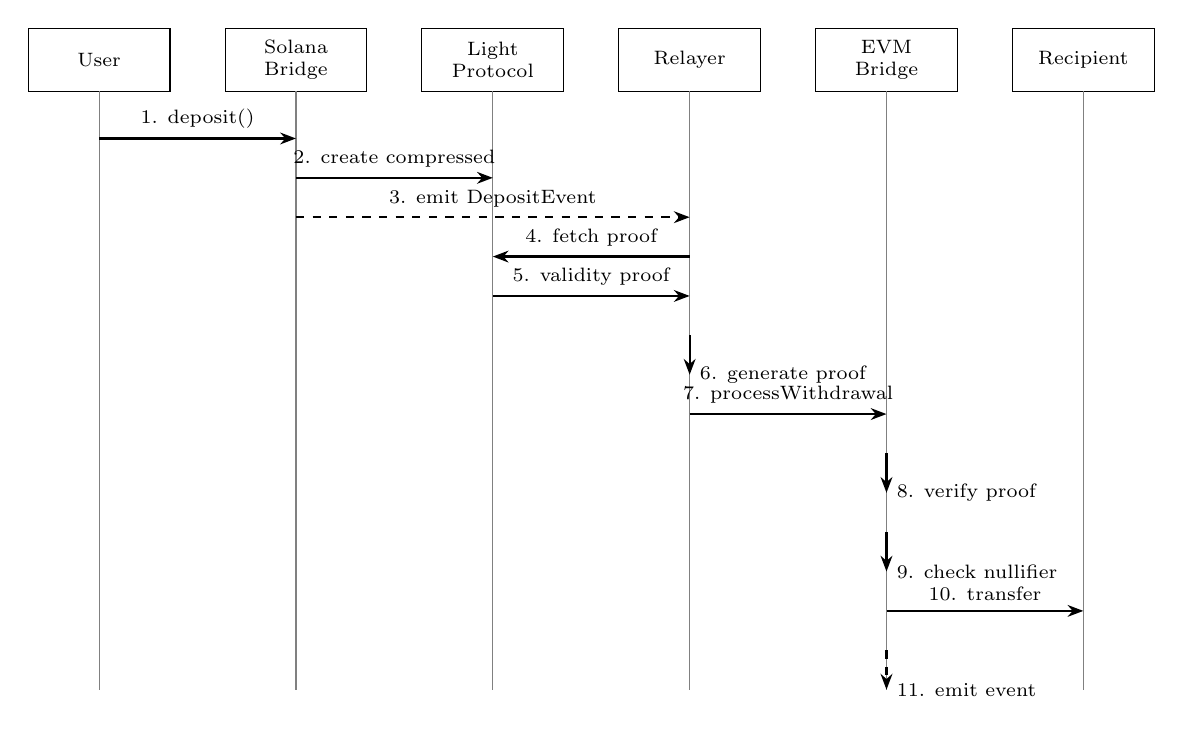
\begin{tikzpicture}[
    participant/.style={draw, minimum width=1.8cm, minimum height=0.8cm, align=center, font=\scriptsize},
    arrow/.style={-{Stealth[length=2mm]}, thick},
    dashedarrow/.style={-{Stealth[length=2mm]}, thick, dashed}
]

% Participants
\node[participant] (user) at (0,0) {User};
\node[participant] (solbridge) at (2.5,0) {Solana\\Bridge};
\node[participant] (light) at (5,0) {Light\\Protocol};
\node[participant] (relayer) at (7.5,0) {Relayer};
\node[participant] (evmbridge) at (10,0) {EVM\\Bridge};
\node[participant] (recipient) at (12.5,0) {Recipient};

% Vertical lines
\foreach \x in {0,2.5,5,7.5,10,12.5} {
    \draw[gray, thin] (\x,-0.4) -- (\x,-8);
}

% Messages
\draw[arrow] (0,-1) -- node[above, font=\scriptsize] {1. deposit()} (2.5,-1);
\draw[arrow] (2.5,-1.5) -- node[above, font=\scriptsize] {2. create compressed} (5,-1.5);
\draw[dashedarrow] (2.5,-2) -- node[above, font=\scriptsize] {3. emit DepositEvent} (7.5,-2);
\draw[arrow] (7.5,-2.5) -- node[above, font=\scriptsize] {4. fetch proof} (5,-2.5);
\draw[arrow] (5,-3) -- node[above, font=\scriptsize] {5. validity proof} (7.5,-3);
\draw[arrow] (7.5,-3.5) -- (7.5,-4) node[right, font=\scriptsize] {6. generate proof};
\draw[arrow] (7.5,-4.5) -- node[above, font=\scriptsize] {7. processWithdrawal} (10,-4.5);
\draw[arrow] (10,-5) -- (10,-5.5) node[right, font=\scriptsize] {8. verify proof};
\draw[arrow] (10,-6) -- (10,-6.5) node[right, font=\scriptsize] {9. check nullifier};
\draw[arrow] (10,-7) -- node[above, font=\scriptsize] {10. transfer} (12.5,-7);
\draw[dashedarrow] (10,-7.5) -- (10,-8) node[right, font=\scriptsize] {11. emit event};

\end{tikzpicture}
\caption{Solana $\rightarrow$ EVM Message Flow}
\label{fig:sol-evm-flow}
\end{figure}

\textbf{Step-by-step breakdown:}
\begin{enumerate}
    \item \textbf{User initiates deposit:} Calls \texttt{deposit(amount, destChainAddr, linkHash)} on Solana bridge
    \item \textbf{Compressed account created:} Light Protocol creates a compressed account with deposit details ($\sim$15,000 lamports)
    \item \textbf{Event emitted:} The Solana program emits a \texttt{DepositEvent} with the compressed account address
    \item \textbf{Relayer fetches proof:} Queries Photon indexer for the validity proof of the compressed account
    \item \textbf{Proof received:} 128-byte validity proof against current state root
    \item \textbf{\groth{} proof generated:} Relayer runs snarkjs with circuit inputs ($\sim$2--5 seconds)
    \item \textbf{Withdrawal submitted:} Relayer calls \texttt{processWithdrawal(record, proof)} on EVM bridge
    \item \textbf{Proof verified:} EVM contract verifies \groth{} proof ($\sim$200,000 gas)
    \item \textbf{Nullifier checked:} Contract confirms nullifier hasn't been used
    \item \textbf{Tokens transferred:} ERC20 tokens sent to recipient address
    \item \textbf{Event emitted:} \texttt{WithdrawalProcessed} event for tracking
\end{enumerate}

\textbf{Total latency:} $\sim$20--25 seconds (5s Solana finality + 2--5s proof gen + 12s EVM confirmation)

\subsection{EVM $\rightarrow$ Solana Transfer}

\begin{figure}[H]
\centering
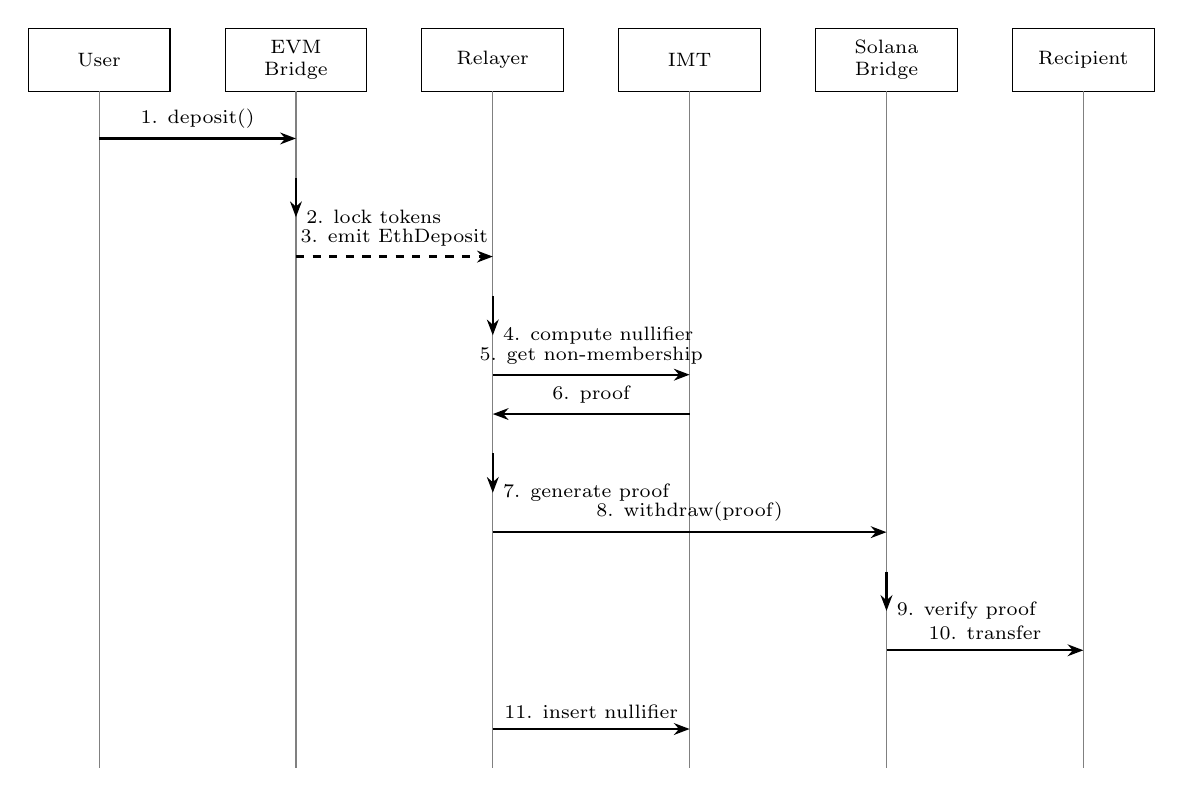
\begin{tikzpicture}[
    participant/.style={draw, minimum width=1.8cm, minimum height=0.8cm, align=center, font=\scriptsize},
    arrow/.style={-{Stealth[length=2mm]}, thick},
    dashedarrow/.style={-{Stealth[length=2mm]}, thick, dashed}
]

% Participants
\node[participant] (user) at (0,0) {User};
\node[participant] (evmbridge) at (2.5,0) {EVM\\Bridge};
\node[participant] (relayer) at (5,0) {Relayer};
\node[participant] (imt) at (7.5,0) {IMT};
\node[participant] (solbridge) at (10,0) {Solana\\Bridge};
\node[participant] (recipient) at (12.5,0) {Recipient};

% Vertical lines
\foreach \x in {0,2.5,5,7.5,10,12.5} {
    \draw[gray, thin] (\x,-0.4) -- (\x,-9);
}

% Messages
\draw[arrow] (0,-1) -- node[above, font=\scriptsize] {1. deposit()} (2.5,-1);
\draw[arrow] (2.5,-1.5) -- (2.5,-2) node[right, font=\scriptsize] {2. lock tokens};
\draw[dashedarrow] (2.5,-2.5) -- node[above, font=\scriptsize] {3. emit EthDeposit} (5,-2.5);
\draw[arrow] (5,-3) -- (5,-3.5) node[right, font=\scriptsize] {4. compute nullifier};
\draw[arrow] (5,-4) -- node[above, font=\scriptsize] {5. get non-membership} (7.5,-4);
\draw[arrow] (7.5,-4.5) -- node[above, font=\scriptsize] {6. proof} (5,-4.5);
\draw[arrow] (5,-5) -- (5,-5.5) node[right, font=\scriptsize] {7. generate proof};
\draw[arrow] (5,-6) -- node[above, font=\scriptsize] {8. withdraw(proof)} (10,-6);
\draw[arrow] (10,-6.5) -- (10,-7) node[right, font=\scriptsize] {9. verify proof};
\draw[arrow] (10,-7.5) -- node[above, font=\scriptsize] {10. transfer} (12.5,-7.5);
\draw[arrow] (5,-8.5) -- node[above, font=\scriptsize] {11. insert nullifier} (7.5,-8.5);

\end{tikzpicture}
\caption{EVM $\rightarrow$ Solana Message Flow}
\label{fig:evm-sol-flow}
\end{figure}

\textbf{Step-by-step breakdown:}
\begin{enumerate}
    \item \textbf{User initiates deposit:} Calls \texttt{deposit()} on EVM bridge contract
    \item \textbf{Tokens locked:} ERC20 tokens transferred to bridge contract
    \item \textbf{Event emitted:} Bridge emits \texttt{EthDeposit} event with deposit details
    \item \textbf{Nullifier computed:} Relayer hashes deposit parameters via $\poseidon_9$
    \item \textbf{Non-membership query:} Relayer queries local IMT to confirm nullifier not present
    \item \textbf{Proof returned:} IMT returns non-membership proof (predecessor/successor linkage)
    \item \textbf{\groth{} proof generated:} Relayer generates IMT insertion proof ($\sim$3--5 seconds)
    \item \textbf{Withdrawal submitted:} Relayer calls \texttt{withdraw(proof, newRoot, nullifier)} on Solana
    \item \textbf{Proof verified:} Solana program verifies \groth{} proof
    \item \textbf{Tokens transferred:} SPL tokens sent to recipient address
    \item \textbf{IMT updated:} Nullifier inserted into local IMT after successful withdrawal
\end{enumerate}

\textbf{Total latency:} $\sim$22--25 seconds (12s EVM confirmation + 3--5s proof gen + 5s Solana finality)

\textbf{Key differences from Solana$\rightarrow$EVM:}
\begin{itemize}
    \item \textbf{Indexed Merkle Tree (IMT):} Used for non-membership proofs (proving nullifier hasn't been used)
    \item \textbf{IMT maintained off-chain:} Relayer stores IMT locally; root hash tracked on Solana
    \item \textbf{Insertion after withdrawal:} Nullifier inserted into IMT only after successful Solana withdrawal
\end{itemize}

% ============================================================================
% SECTION 7: FAILURE CASES
% ============================================================================
\section{Failure Cases and Recovery}
\label{sec:failures}

\subsection{Network Failures}

\subsubsection{RPC Unavailability}
\textbf{Scenario:} Solana or EVM RPC endpoints become unreachable.

\textbf{Impact:} Relayer cannot fetch events or submit transactions.

\textbf{Recovery:}
\begin{itemize}
    \item Relayer implements exponential backoff retry logic
    \item Multiple RPC endpoints configured as fallbacks
    \item User funds remain safe in source chain contracts
\end{itemize}

\subsubsection{Block Reorganization}
\textbf{Scenario:} A confirmed block is reverted due to chain reorganization.

\textbf{Impact:} Deposit events may be ``undone'' if processed before finality.

\textbf{Mitigation:}
\begin{itemize}
    \item Relayer waits for finalized commitment on Solana ($\sim$15--30 seconds)
    \item Relayer waits for sufficient confirmations on EVM (12+ blocks)
    \item Deposits processed only after achieving finality threshold
\end{itemize}

\subsection{Relayer Failures}

\subsubsection{Relayer Downtime}
\textbf{Scenario:} Relayer service crashes or becomes unresponsive.

\textbf{Impact:} Deposits are not processed; funds remain locked.

\textbf{Recovery:}
\begin{enumerate}
    \item \textbf{Time-lock mechanism:} Deposits have a maximum processing window (e.g., 24 hours)
    \item \textbf{User reclaim:} After time-lock expiry, users can call \texttt{reclaimDeposit()} on source chain
    \item \textbf{No fund loss:} Funds are never permanently stuck
\end{enumerate}

\subsubsection{Relayer Compromise}
\textbf{Scenario:} Attacker gains control of relayer private keys.

\textbf{Impact:} Limited to denial of service.

\textbf{Why funds are safe:}
\begin{itemize}
    \item Cannot forge \groth{} proofs (requires valid witness)
    \item Cannot modify withdrawal amounts (verified by circuit)
    \item Cannot double-spend (nullifiers tracked on-chain)
    \item Can only refuse to process (liveness attack, not safety)
\end{itemize}

\subsection{Recovery Matrix}

\begin{table}[H]
\centering
\caption{Failure Recovery Matrix}
\label{tab:recovery}
\begin{tabular}{@{}llll@{}}
\toprule
\textbf{Failure Mode} & \textbf{Impact} & \textbf{User Action} & \textbf{Recovery Time} \\
\midrule
RPC down & Delayed processing & None & Minutes \\
Block reorg & Potential retry & None & Minutes \\
Relayer down & Stuck deposits & Reclaim after timeout & Hours \\
Relayer compromise & DoS only & Wait for recovery & Hours \\
Tree full & New deposits fail & None (auto-rollover) & Minutes \\
Queue full & New deposits fail & None (forester catches up) & Hours \\
\bottomrule
\end{tabular}
\end{table}

% ============================================================================
% SECTION 8: GAS, LATENCY, FINALITY
% ============================================================================
\section{Gas, Latency, and Finality}
\label{sec:performance}

\subsection{Cost Analysis}

\subsubsection{Solana Costs}

\begin{table}[H]
\centering
\caption{Solana Operation Costs}
\label{tab:solana-costs}
\begin{tabular}{@{}llll@{}}
\toprule
\textbf{Operation} & \textbf{Traditional} & \textbf{Compressed} & \textbf{Savings} \\
\midrule
Create deposit record & $\sim$1,600,000 lamports & $\sim$15,000 lamports & 99.06\% \\
Create token account & $\sim$2,000,000 lamports & $\sim$5,000 lamports & 99.75\% \\
Store nullifier & $\sim$890,880 lamports & $\sim$15,000 lamports & 98.32\% \\
Transaction fee & $\sim$5,000 lamports & $\sim$5,000 lamports & 0\% \\
\bottomrule
\end{tabular}
\end{table}

\textbf{Total deposit cost (Solana side):} $\sim$20,000 lamports ($\sim$\$0.003 at SOL=\$150)

\subsubsection{EVM Costs}

\begin{table}[H]
\centering
\caption{EVM Operation Costs}
\label{tab:evm-costs}
\begin{tabular}{@{}lll@{}}
\toprule
\textbf{Operation} & \textbf{Gas Used} & \textbf{Cost @ 30 gwei} \\
\midrule
\groth{} verification & $\sim$200,000 & $\sim$\$3--5 \\
Nullifier storage & $\sim$20,000 & $\sim$\$0.30 \\
ERC20 transfer & $\sim$65,000 & $\sim$\$1 \\
Event emission & $\sim$5,000 & $\sim$\$0.08 \\
\midrule
\textbf{Total withdrawal} & $\sim$\textbf{290,000} & $\sim$\textbf{\$4--6} \\
\bottomrule
\end{tabular}
\end{table}

\textbf{Note:} Costs vary significantly based on network congestion and gas prices.

\subsubsection{Fee Model}

The relayer deducts fees from the transfer amount:

\begin{equation}
\text{net\_amount} = \text{gross\_amount} - \text{gas\_fee} - \text{relayer\_fee} - \text{LP\_fee}
\end{equation}

Where:
\begin{itemize}
    \item \textbf{gas\_fee:} Estimated destination chain transaction cost
    \item \textbf{relayer\_fee:} Flat fee for relayer infrastructure ($\sim$\$0.50)
    \item \textbf{LP\_fee:} Liquidity provider incentive (0.1\% of amount)
\end{itemize}

\textbf{Example:} 1000 USDC transfer, Solana$\rightarrow$Ethereum
\begin{itemize}
    \item Gas fee: $\sim$\$5.00
    \item Relayer fee: \$0.50
    \item LP fee: \$1.00
    \item \textbf{Net received:} 993.50 USDC
\end{itemize}

\subsection{Latency Analysis}

\subsubsection{Solana Commitment Levels}

\begin{table}[H]
\centering
\caption{Solana Commitment Levels}
\label{tab:solana-commitment}
\begin{tabular}{@{}lll@{}}
\toprule
\textbf{Level} & \textbf{Time} & \textbf{Security} \\
\midrule
Processed & $\sim$400ms & Single validator confirmation \\
Confirmed & $\sim$2--3s & Supermajority (66\%+) vote \\
Finalized & $\sim$15--30s & 31+ confirmed blocks \\
\bottomrule
\end{tabular}
\end{table}

\protocol{} waits for \textbf{finalized} commitment to ensure deposit cannot be reverted.

\subsubsection{End-to-End Latency}

\textbf{Solana $\rightarrow$ EVM:}
\begin{table}[H]
\centering
\begin{tabular}{@{}ll@{}}
\toprule
\textbf{Stage} & \textbf{Duration} \\
\midrule
Solana deposit confirmation & $\sim$5s (finalized) \\
Event detection & $\sim$1s \\
Proof generation (snarkjs) & $\sim$2--5s \\
EVM transaction broadcast & $\sim$1s \\
EVM confirmation & $\sim$12s (1 block) \\
\midrule
\textbf{Total} & $\sim$\textbf{20--25s} \\
\bottomrule
\end{tabular}
\end{table}

\subsection{Throughput Considerations}

\subsubsection{Sequential Processing Limitation}

Current implementation uses \textbf{Indexed Merkle Trees} which require sequential updates:
\begin{itemize}
    \item Each IMT insertion depends on the previous root
    \item Parallel withdrawals would create conflicting root updates
    \item Theoretical maximum: $\sim$1 withdrawal per proof generation cycle ($\sim$3--5s)
\end{itemize}

\textbf{Practical throughput:} $\sim$12--20 withdrawals per minute per direction

\subsubsection{Future Optimization: Concurrent Merkle Trees}

Light Protocol supports \textbf{Concurrent Merkle Trees}~[16] which allow parallel updates:
\begin{itemize}
    \item Multiple proofs can reference the same root
    \item Conflicts resolved via changelog mechanism
    \item Theoretical improvement: 10--100x throughput
\end{itemize}

This optimization is planned for future releases.

% ============================================================================
% SECTION 9: COMPARISON
% ============================================================================
\section{Comparison with Existing Solutions}
\label{sec:comparison}

\subsection{Feature Comparison Matrix}

\begin{table}[H]
\centering
\caption{Feature Comparison with Existing Bridges}
\label{tab:comparison}
\small
\begin{tabular}{@{}llllll@{}}
\toprule
\textbf{Feature} & \textbf{Meridian Link} & \textbf{Wormhole} & \textbf{LayerZero} & \textbf{deBridge} & \textbf{Allbridge} \\
\midrule
Trust Model & ZK Proofs & 13/19 Guardians & Oracle + DVN & Validators & Pool Ops \\
Verification & Groth16 & ECDSA Sigs & ECDSA Sigs & ECDSA Sigs & Centralized \\
Wrapped Tokens & No & Yes & Configurable & No & No \\
Storage & Compressed & Full accounts & Minimal & Minimal & Pool state \\
Latency & $\sim$20--25s & 15--20 min & Variable & Real-time & Fast \\
User Recovery & Time-lock & Guardian & DVN-dependent & Support & Support \\
Solana Support & Native & Native & Via adapters & Native & Native \\
TVL & N/A (new) & $\sim$\$2B & N/A & Growing & $\sim$\$25M \\
\bottomrule
\end{tabular}
\end{table}

\subsection{Security Model Analysis}

Each bridge makes different trust assumptions. We characterize them by their \textbf{security bottleneck}:

\begin{table}[H]
\centering
\caption{Security Bottleneck Analysis}
\label{tab:security-bottleneck}
\begin{tabular}{@{}lll@{}}
\toprule
\textbf{Bridge} & \textbf{Security Bottleneck} & \textbf{Attack Threshold} \\
\midrule
Wormhole & Guardian honesty & 7/19 compromised guardians \\
LayerZero & DVN + Oracle honesty & Application-dependent \\
deBridge & Validator honesty & Validator set compromise \\
Allbridge & Pool operator honesty & Single operator compromise \\
\protocol{} & Groth16 + trusted setup & $\sim 2^{-100}$ forgery probability \\
\bottomrule
\end{tabular}
\end{table}

\textbf{Honest assessment of \protocol{}:}

\textit{Strengths over signature-based bridges:}
\begin{itemize}
    \item Relayer cannot forge proofs (cryptographic, not economic security)
    \item User recovery via time-lock (no intermediary required)
    \item No wrapped tokens (native asset transfers)
\end{itemize}

\textit{Weaknesses compared to established bridges:}
\begin{itemize}
    \item Trusted setup introduces systemic risk if ceremony compromised
    \item Lower throughput ($\sim$12--20/min vs. unlimited for signature verification)
    \item Less battle-tested (new protocol)
    \item Higher EVM costs (\$4--6) than some competitors (\$2--5)
\end{itemize}

\subsection{Cost and Latency Summary}

\begin{table}[H]
\centering
\caption{Cost and Latency Comparison}
\label{tab:cost-latency}
\begin{tabular}{@{}llll@{}}
\toprule
\textbf{Bridge} & \textbf{Total Cost (1000 USDC)} & \textbf{Latency} & \textbf{Throughput} \\
\midrule
Wormhole & $\sim$\$5--11 & 15--20 min & High \\
LayerZero & $\sim$\$3--9 & Variable & High \\
deBridge & $\sim$\$2--6 & 30s--2 min & High \\
Allbridge & $\sim$\$5--15 & 1--5 min & Medium \\
\textbf{\protocol{}} & $\sim$\textbf{\$4--7} & \textbf{20--25s} & \textbf{Low ($\sim$12--20/min)} \\
\bottomrule
\end{tabular}
\end{table}

\textbf{Honest cost analysis:} \protocol{}'s Solana storage savings ($\sim$\$0.007/deposit) are meaningful at scale but negligible for individual users. EVM verification costs dominate. For transfers under \$500, the $\sim$\$5 fee represents 1\%+ of value.

% ============================================================================
% SECTION 10: FUTURE WORK
% ============================================================================
\section{Future Work}
\label{sec:future}

\subsection{Near-Term (0--6 months)}

\subsubsection{Mainnet Deployment}
The current implementation operates on Solana devnet and Ethereum Sepolia testnet. Mainnet deployment requires:
\begin{itemize}
    \item \textbf{Security audit:} Comprehensive audit of smart contracts and circuits
    \item \textbf{Trusted setup ceremony:} Production \groth{} keys via multi-party computation
    \item \textbf{Gradual rollout:} Start with low limits, increase based on monitoring
    \item \textbf{Bug bounty program:} Incentivize security researchers
\end{itemize}

\subsubsection{Fee Structure and Rate Limiting}
Implement on-chain fee configuration with base fees, percentage fees, and transfer limits to manage liquidity and incentivize relayer operation.

\subsubsection{Additional Chain Support}
Priority EVM chains: Arbitrum One, Base, HyperLiquid, Optimism, Polygon zkEVM

\subsection{Medium-Term (6--18 months)}

\subsubsection{Concurrent Merkle Trees}
Replace Indexed Merkle Trees with Concurrent Merkle Trees~[16]:
\begin{itemize}
    \item \textbf{Parallel processing:} Multiple withdrawals processed simultaneously
    \item \textbf{Throughput improvement:} 10--100x increase in transactions per second
    \item \textbf{Backward compatible:} Existing nullifiers remain valid
\end{itemize}

\subsubsection{Hardware-Accelerated Proving}
Integrate GPU/FPGA acceleration for proof generation:
\begin{itemize}
    \item \textbf{Current:} $\sim$2--5s proof generation (CPU, snarkjs)
    \item \textbf{Target:} $\sim$100--500ms proof generation (GPU, rapidsnark)
    \item \textbf{Benefit:} Reduced latency, higher throughput
\end{itemize}

\subsubsection{Decentralized Relayer Network}
Transition from single relayer to permissionless network with staking requirements. Open research questions include:
\begin{itemize}
    \item \textbf{Incentive design:} How to reward liveness without enabling MEV extraction
    \item \textbf{Slashing conditions:} What constitutes slashable behavior when proof forgery is cryptographically impossible
    \item \textbf{Coordination:} How multiple relayers avoid duplicate proof submissions
\end{itemize}

% ============================================================================
% SECTION 11: CONCLUSION
% ============================================================================
\section{Conclusion}
\label{sec:conclusion}

\protocol{} presents an alternative approach to cross-chain bridging that shifts trust assumptions from signature-based attestation to zero-knowledge proof verification, combined with state compression for cost efficiency.

\subsection{Contributions}

\begin{enumerate}
    \item \textbf{Cost Reduction:} Light Protocol state compression reduces Solana storage costs by $\sim$99\% per deposit record ($\sim$15K vs $\sim$1.6M lamports). However, EVM verification costs ($\sim$\$4--6) dominate total transfer cost for typical transactions.
    
    \item \textbf{Verification Model:} \groth{} proofs replace multisig/oracle attestation. Safety (no fund theft) holds under $\sim$100-bit BN254 security and trusted setup integrity. Liveness depends on relayer operation.
    
    \item \textbf{Replay Protection:} \poseidon{}-based nullifiers with on-chain tracking prevent double-spending without centralized databases.
    
    \item \textbf{User Recovery:} Time-lock mechanism allows users to reclaim deposits if relayer fails, eliminating permanent fund loss scenarios (assuming contract remains accessible).
\end{enumerate}

\subsection{Limitations and Trade-offs}

\begin{table}[H]
\centering
\caption{Limitations and Mitigations}
\label{tab:limitations}
\begin{tabular}{@{}lll@{}}
\toprule
\textbf{Trade-off} & \textbf{Impact} & \textbf{Mitigation} \\
\midrule
Trusted setup & Proof forgery if compromised & Multi-party computation \\
Throughput & $\sim$12--20 withdrawals/min & Concurrent Merkle Trees \\
EVM costs & $\sim$\$4--6 per withdrawal & Batching, L2 deployment \\
Proof latency & $\sim$2--5s added per transfer & Hardware acceleration \\
Relayer centralization & Censorship, MEV possible & Decentralized network \\
New protocol & Limited battle-testing & Audits, gradual rollout \\
\bottomrule
\end{tabular}
\end{table}

\subsection{Open Questions}

Several aspects warrant further research and discussion:
\begin{enumerate}
    \item \textbf{Circuit upgradeability:} How can circuits be upgraded without breaking existing deposits in flight?
    \item \textbf{Proof aggregation:} Can multiple withdrawal proofs be batched to reduce per-transaction EVM costs?
\end{enumerate}

\subsection{Invitation}

This protocol is open-source. We welcome technical review, security analysis, and implementation contributions. The codebase is available at the repository linked below.

% ============================================================================
% REFERENCES
% ============================================================================
\newpage
\section*{References}
\addcontentsline{toc}{section}{References}

\begin{enumerate}[label={[\arabic*]}]
    \item \label{solana-rent} Solana Documentation. ``Rent.'' \url{https://docs.solana.com/developing/intro/rent}
    
    \item \label{light-protocol} Light Protocol. ``ZK Compression Whitepaper.'' \url{https://www.zkcompression.com/references/whitepaper}
    
    \item \label{wormhole} Wormhole. ``Wormhole Whitepaper.'' \url{https://wormhole.com/whitepaper.pdf}
    
    \item \label{layerzero} LayerZero. ``LayerZero V2 Whitepaper.'' \url{https://layerzero.network/publications/LayerZero_Whitepaper_V2.0.0.pdf}
    
    \item \label{groth16} Groth, Jens. ``On the size of pairing-based non-interactive arguments.'' \textit{Advances in Cryptology--EUROCRYPT 2016}.
    
    \item \label{poseidon} Grassi, Lorenzo, et al. ``Poseidon: A new hash function for zero-knowledge proof systems.'' \textit{USENIX Security 2021}.
    
    \item \label{bls12-381} Bowe, Sean. ``BLS12-381: New zk-SNARK Elliptic Curve Construction.'' \textit{Zcash Blog}, 2017.
    
    \item \label{solana-whitepaper} Yakovenko, Anatoly. ``Solana: A new architecture for a high performance blockchain.'' \textit{Solana Whitepaper}, 2017.
    
    \item \label{gasper} Buterin, Vitalik, et al. ``Combining GHOST and Casper.'' \textit{arXiv:2003.03052}, 2020.
    
    \item \label{eip196} Ethereum Foundation. ``EIP-196: Precompiled contracts for addition and scalar multiplication on the elliptic curve alt\_bn128.'' 2017.
    
    \item \label{solana-tx} Solana Documentation. ``Transaction Size Limits.'' \url{https://docs.solana.com/developing/programming-model/transactions}
    
    \item \label{wormhole-rekt} Rekt News. ``Wormhole - REKT.'' \url{https://rekt.news/wormhole-rekt/}, February 2022.
    
    \item \label{debridge} deBridge. ``deBridge Documentation.'' \url{https://docs.debridge.finance/}
    
    \item \label{allbridge} Allbridge. ``Allbridge Core Documentation.'' \url{https://docs.allbridge.io/}
    
    \item \label{imt} Aztec Protocol. ``Indexed Merkle Tree.'' \url{https://docs.aztec.network/aztec/concepts/storage/trees/indexed_merkle_tree}
    
    \item \label{cmt} Solana Documentation. ``Concurrent Merkle Trees.'' \url{https://solana.com/developers/guides/javascript/compressed-nfts}
    
    \item \label{kim-barbulescu} Kim, Taechan and Barbulescu, Razvan. ``Extended Tower Number Field Sieve: A New Complexity for the Medium Prime Case.'' \textit{CRYPTO 2016}.
\end{enumerate}

% ============================================================================
% APPENDIX
% ============================================================================
\newpage
\appendix
\section{Cryptographic Primitives}
\label{app:crypto}

\subsection{Poseidon Hash Function}

\poseidon{}~[6] is an algebraic hash function optimized for zero-knowledge proof systems:
\begin{itemize}
    \item \textbf{Field:} BN254 scalar field (prime $\sim 2^{254}$)
    \item \textbf{Width:} Configurable (we use 7-ary for nullifiers, 2-ary for Merkle trees)
    \item \textbf{Rounds:} Full rounds + partial rounds (security parameter dependent)
    \item \textbf{Constraints:} $\sim$300 R1CS constraints per hash (vs $\sim$25,000 for SHA-256)
\end{itemize}

\subsection{Groth16 Proof System}

\groth{}~[5] provides succinct non-interactive arguments of knowledge (SNARKs):
\begin{itemize}
    \item \textbf{Proof size:} 256 bytes (constant)
    \item \textbf{Verification:} 6 pairing operations ($\sim$200K gas on EVM)
    \item \textbf{Security:} $\sim$100--110 bit on BN254 (see Section~\ref{sec:security} for discussion)
    \item \textbf{Trusted setup:} Circuit-specific (phase 1: powers of tau, phase 2: circuit specific)
\end{itemize}

\subsection{BN254 Curve Parameters}

The BN254 (alt\_bn128) curve used in Circom:
\begin{align*}
p &= 21888242871839275222246405745257275088696311157297823662689037894645226208583 \\
r &= 21888242871839275222246405745257275088548364400416034343698204186575808495617
\end{align*}

EVM precompiles (EIP-196, EIP-197) provide efficient operations on this curve.

\section{Circuit Specifications}
\label{app:circuits}

\subsection{Solana Deposit Proof Circuit}

\begin{table}[H]
\centering
\begin{tabular}{@{}ll@{}}
\toprule
\textbf{Parameter} & \textbf{Value} \\
\midrule
Merkle tree depth & 26 \\
Public inputs & 4 (stateRoot, amount, destChainId, destChainAddr) \\
Private inputs & 13 \\
Public outputs & 3 (nullifier, commitment, isValid) \\
Constraints & $\sim$15,000 R1CS \\
Proving time & $\sim$2--5s (CPU) \\
Proof size & 256 bytes \\
\bottomrule
\end{tabular}
\end{table}

\subsection{Ethereum Deposit Proof Circuit}

\begin{table}[H]
\centering
\begin{tabular}{@{}ll@{}}
\toprule
\textbf{Parameter} & \textbf{Value} \\
\midrule
IMT depth & 32 \\
Public inputs & 10 (deposit event fields) \\
Private inputs & 5 (IMT proof data) \\
Public outputs & 2 (nullifier, newRoot) \\
Constraints & $\sim$20,000 R1CS \\
Proving time & $\sim$3--5s (CPU) \\
Proof size & 256 bytes \\
\bottomrule
\end{tabular}
\end{table}

% ============================================================================
% DOCUMENT INFO
% ============================================================================
\vfill
\begin{center}
\rule{0.5\textwidth}{0.4pt}

\textbf{Document Version:} 1.0 \\
\textbf{Last Updated:} January 2026 \\
\textbf{License:} MIT \\
\textbf{Repository:} \url{https://github.com/RippnerLabs/meridian-link}
\end{center}

\end{document}
